\chapter{Prototipo 2: Visualizar los datos en recomendaciones por contenido}
  \section{Análisis}
    \subsection{Objetivo}
      Visualizar recomendaciones bajo el filtrado por contenido de los platillos contenidos en el sistema. 

    \subsection{Características}
    \begin{itemize}
      \item El sistema permite al usuario visualizar los platillos.
      \item El sistema muestra recomendaciones de acuerdo a un solo platillo, para mostrar los que tienen una mayor similitud con éste.
      \item El sistema permite la interacción de usuarios no registrados para obtener recomendaciones personalizadas con base en los platillos que ha visualizado.
      \item La evaluación de similitud se logra a través de las categorías en común que tengan los platillos entre sí.
    \end{itemize}

    \subsection{Restricciones}
    \begin{itemize}
      \item El sistema se ve limitado a la cantidad y características de los platillos existentes actualmente.
      \item El usuario no registrado no podrá modificar o eliminar los platillos del sistema.
    \end{itemize}

  \section{Diseño}
    Para la implementación de las recomendaciones por contenido, se consideran las categorías que tienen en común. La cantidad de categorías que poseen en común es identificada por una evaluación de similitud. Dicha evaluación genera un conjunto de relaciones con las que es posible determinar los artículos que se parecen más entre sí y obtener los vecinos más cercanos a cada elemento. Así, para los platillos, las categorías a las que pertenecen, permiten crear una vecindad para cada nodo donde es posible obtener cuáles son los platillos vecinos que más se parecen entre sí.

    \subsection{Diagrama de clases}
    Implementando el comportamiento descrito anteriormente se generan las clases mostradas en la figura~\ref{fig: diagrama clases p2} que permiten obtener las recomendaciones por contenido. 
          \begin{figure}[h!]
          \centering
          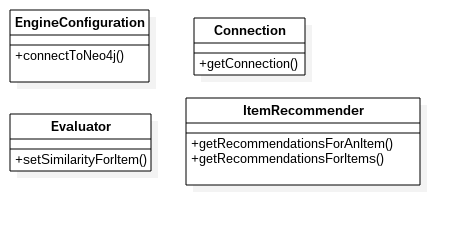
\includegraphics[width=12cm]{./images/p2_classes.png}
          \caption{Diagrama de clases del prototipo 2}
          \label{fig: diagrama clases p2}
        \end{figure}

    \subsection{Casos de uso}
    Integrando la funcionalidad planteada en las clases anteriores dentro de un sistema web que permita la interacción del usuario se plantean los siguientes casos de uso mostrados en la figura~\ref{fig:CU p2}
    \begin{figure}[h!]
      \centering
      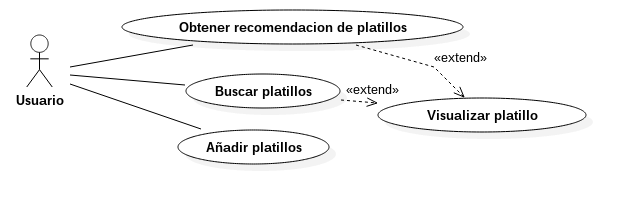
\includegraphics[width=16cm]{./images/prototipo2.png}
      \caption{Casos de uso del prototipo 2}
      \label{fig:CU p2}
    \end{figure}
    
    \paragraph{CU. Obtener recomendación de platillos\\} 
    \textbf{Descripción:} El usuario obtiene recomendaciones del sistema\\
    \textbf{Actores:} Usuario \\
    \textbf{Precondiciones:} Ninguna \\
    \textbf{Flujo normal}\\
    \begin{itemize}
      \item El sistema muestra información de platillos relevantes no personalizadas.
    \end{itemize}
    \textbf{Flujo alternativo}\\
    \begin{itemize}
      \item El sistema muestra recomendaciones personalizadas de acuerdo a interacciones previas del usuario.
    \end{itemize}

    \paragraph{CU. Buscar platillos\\}
    \textbf{Descripción:} El usuario utiliza el sistema de búsqueda para encontrar platillos relacionados.\\
    \textbf{Actores:} Usuario\\
    \textbf{Precondiciones:} Ninguna\\
    \textbf{Flujo normal}\\
    \begin{itemize}
      \item El usuario escribe su búsqueda en el sistema. 
      \item El sistema obtiene los platillos encontrados, así como platillos relacionados
      \item El sistema muestra los resultados al usuario
    \end{itemize}

    \paragraph{CU. Visualizar platillo\\}
    \textbf{Descripción:} El usuario visualiza la información descriptiva de un platillo\\
    \textbf{Actores:} Usuario\\
    \textbf{Precondiciones:} El usuario selecciona un platillo desde el CU. Obtener recomendación de platillos o desde el CU. Buscar platillos\\
    \textbf{Flujo normal}\\
    \begin{itemize}
      \item El usuario selecciona un platillo de la lista de resultados
      \item El sistema muestra la información descriptiva de ese platillo.
    \end{itemize}

    \paragraph{CU. Agregar platillo\\}
    \textbf{Descripción:} El usuario agrega un platillo en el sistema\\
    \textbf{Actores:} Usuario\\
    \textbf{Precondiciones:} Ninguna\\
    \textbf{Flujo normal}\\
    \begin{itemize}
      \item El sistema muestra el método de entrada para las características de los platillos
      \item El usuario introduce los parámetros necesarios para registrar el platillo. (Nombre, descripción y categorías a las que pertenece)
      \item El sistema carga la información del platillo al sistema.
    \end{itemize}
    \textbf{Flujo alternativo}\\
    \begin{itemize}
      \item El sistema comprueba la validez de los datos, si no son correctos, se avisa al actor permitiendo que se corrijan. 
      \item Si el sistema no puede salvar la información del nuevo platillo, se notifica al usuario que el platillo no ha sido agregado.
    \end{itemize}
    
  \section{Resultados}
    Tras definir las acciones realizadas en el prototipo, se realiza el desarrollo del sistema Bonappettit, prototipo del sistema final que permite obtener recomendaciones con filtrado por contenido para usuarios no registrados en la plataforma. Esta plataforma se ve implementada en un sistema web cuyo estilo visual es posible de apreciar en la figura~\ref{fig: screenshot1 p2}
        \begin{figure}[h!]
          \centering
          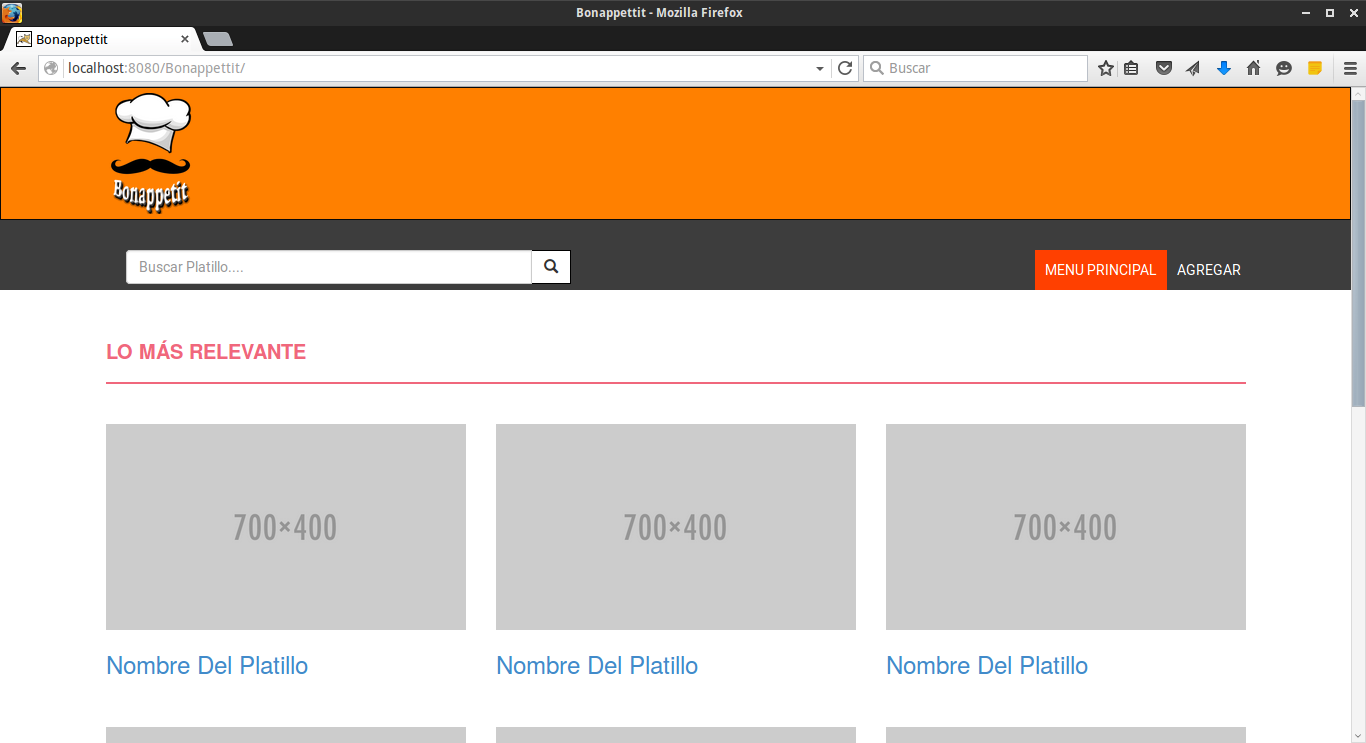
\includegraphics[width=16cm]{./images/bonappettit.png}
          \caption{Capturas de pantalla del sistema}
          \label{fig: screenshot1 p2}
        \end{figure}

    Así mismo, podemos denotar el resultado de las recomendaciones para un ítem en particular como prueba de la implementación del algoritmo k-NN implementado para reconocer la similitud entre los diversos platillos que se encuentran registrados en el sistema, como se describió en el diseño del prototipo. Debido a la ausencia de usuarios registrados en el sistema, y a la falta de información de restaurantes de una zona en particular, el prototipo se ve limitado a recomendar platillos de acuerdo a sus categorías por filtrado por contenido. Actualmente se cuenta con registro de 843 platillos dentro de la base de datos disponibles para hacer pruebas con las recomendaciones necesarias, se espera este número aumente con el tiempo. Por lo mismo, del modelo de datos propuesto para el caso de estudio en la figura~\ref{fig:data model}, para este prototipo se ve limitado al modelo observado en la figura~\ref{fig:p2 db} solo permitiendo la recomendación de platillos. Como prueba de su funcionamiento, la figura~\ref{fig:screenshot2 p2} muestra el resultado de la recomendación para la búsqueda de ensaladas, de acuerdo a las características denotadas por las categorías a las que pertenece el primer platillo encontrado. 

      \begin{figure}[h!]
          \centering
          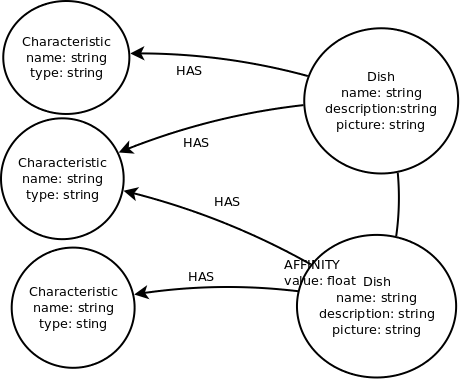
\includegraphics[width=16cm]{./images/p2_model}
          \caption{Modelo de datos con funcionalidad limitada para el prototipo 2}
          \label{fig:p2 db}
        \end{figure}

        \begin{figure}[h!]
          \centering
          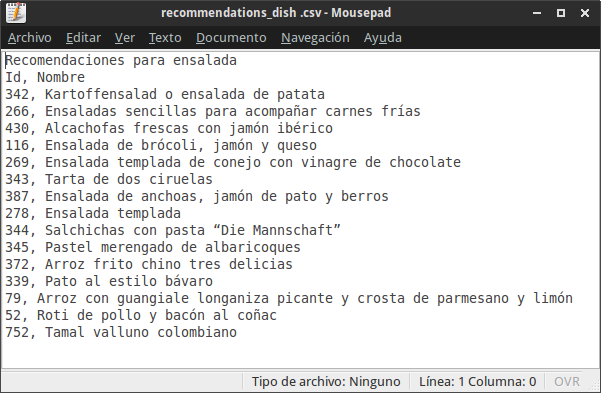
\includegraphics[width=16cm]{./images/recommendations_dish}
          \caption{Recomendación obtenida para la búsqueda de ensaladas}
          \label{fig:screenshot2 p2}
        \end{figure}